\chapter{Literature Review}
\label{chap:litreview}
	\section{Introduction}
		In order to understand the need for a clinical method of detecting deep tissue injuries, the full scope and current state of the issue must be explored. To this end, the current state of the literature regarding deep tissue injuries, how they form, what factors characterize them, and how they are currently treated is explored here. In order to relate this disease to the detection modality proposed in this work, the mechanics and history of ultrasound elastography are also explored and related back to the problem at hand. The major gaps in the current literature regarding the use of ultrasound elastography for detecting and monitoring deep tissue injuries are presented as these gaps are what this work attempts to begin to fill.

	\section{Deep Tissue Injuries}
		Pressure ulcers, commonly referred to as ``bedsores'', are an extraordinarily large problem facing the health care system today. At least \unit{\$3.3}{billion} is spent in the United States of America alone treating approximately 500,000 injuries annually \cite{beckrich99,russo08} while only a minute fraction of that is spent toward pressure ulcer research \cite{zanca03}. Compared to hospital stays for all other conditions, patients with at least a secondary diagnosis of a pressure ulcer were more often discharged to a long-term care facility and more likely resulted in death \cite{russo08}. These injuries place an extremely significant burden on the people who suffer from them---pressure ulcers were found to have a profound impact on people's lives including: altering their physical, social, and financial status; changing their body image; losing independence and control; and subjecting them to the grieving process \cite{langemo00,baharestani94}. \note[KH]{I already mentioned this in the introduction, verbatim. Where should it go?}These debilitating wounds are often suffered by people with limited mobility such as those undergoing lengthy surgical procedures, the elderly, and those with spinal cord injuries (SCI) \cite{allman95}---approximately \unit{80}{\%} of people with spinal cord injuries (SCI) will develop at least one pressure ulcer during their lifetime \cite{salzberg96} and approximately \unit{19}{\%} of elderly patients in long-term care facilities will develop one \cite{freitas11}. Pressure ulcers exist throughout the entire health-care system and are often formed when undergoing hospitalization \cite{aronovitch99}. These injuries have a tendency to become chronic, non-healing wounds and many patients die from complications related to them \cite{jaul10}. Further, patients who have developed at least one pressure ulcer in their life are at a significantly greater risk of developing a second \cite{niazi97}. Pressure ulcers and deep tissue injuries generally form at the bone-muscle interface deep in the tissue \cite{kanno09} with approximately \unit{64}{\%} occurring over the ischial tuberosities, trochanter, or sacrum \cite{garber03}. In general, these injuries are characterized by a some manner of tissue loss through necrosis of the tissue, though there is currently some debate on the exact nature of these wounds as well as the accuracy of the clinical descriptions attributed to them by the National Pressure Ulcer Advisory Panel (NPUAP).

		The NPUAP defines pressure ulcers as a ``localized injury to the skin and / or underlying tissue usually over a bony prominence, as a result of pressure, or pressure in combination with shear and / or friction'' and are generally staged according to a tiered system of increasing damage \cite{npuap07}. The various stages are depicted in Fig. \ref{fig:npuap-staging} and described as follows:

		\begin{figure*}[!t]
			\centering
			\subfloat[Normal tissue]{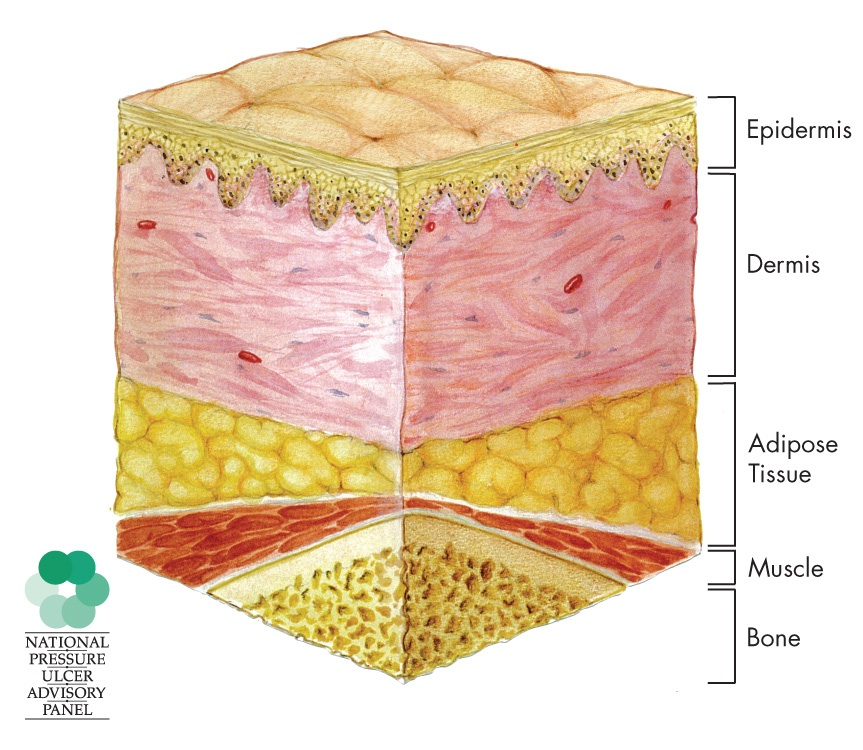
\includegraphics[width=0.3\textwidth]{images/npuap/normal.png}\label{fig:npuap-normal}}

			\subfloat[Stage I]{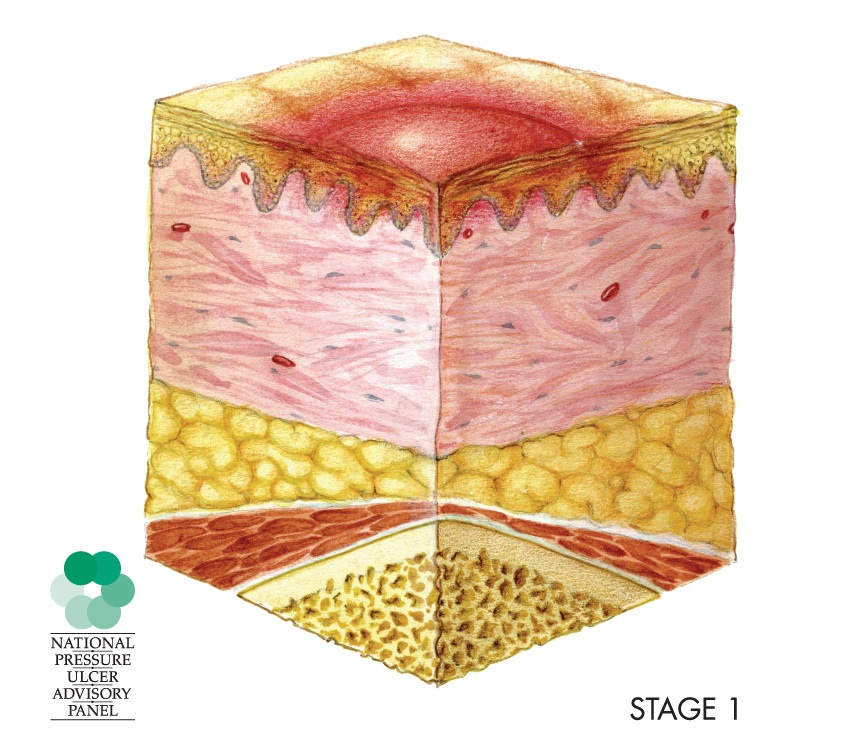
\includegraphics[width=0.3\textwidth]{images/npuap/stage1.png}\label{fig:npuap-stage1}}
			\subfloat[Stage II]{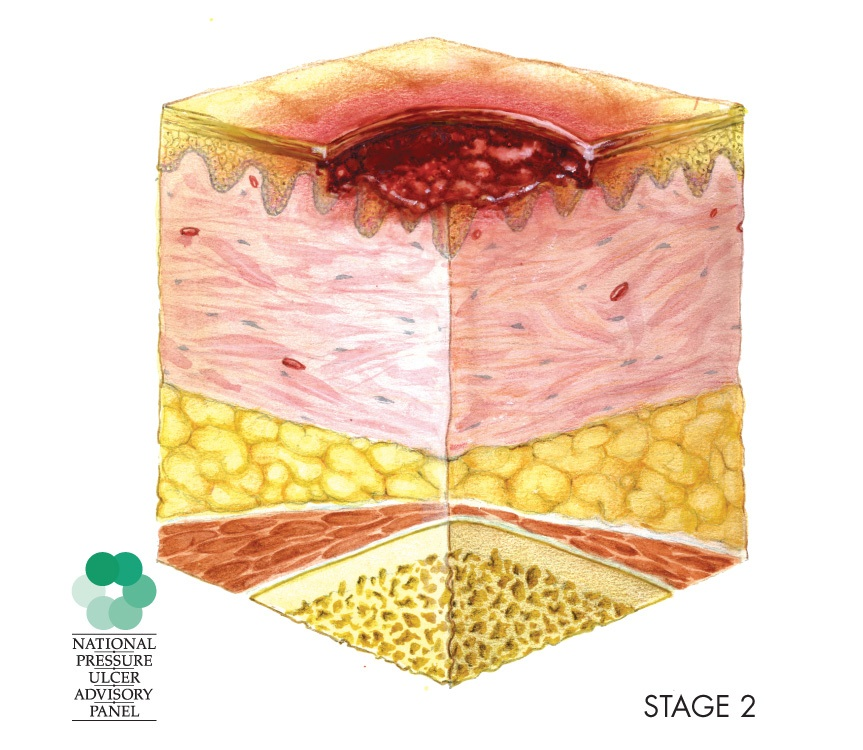
\includegraphics[width=0.3\textwidth]{images/npuap/stage2.png}\label{fig:npuap-stage2}}
			\subfloat[Stage III]{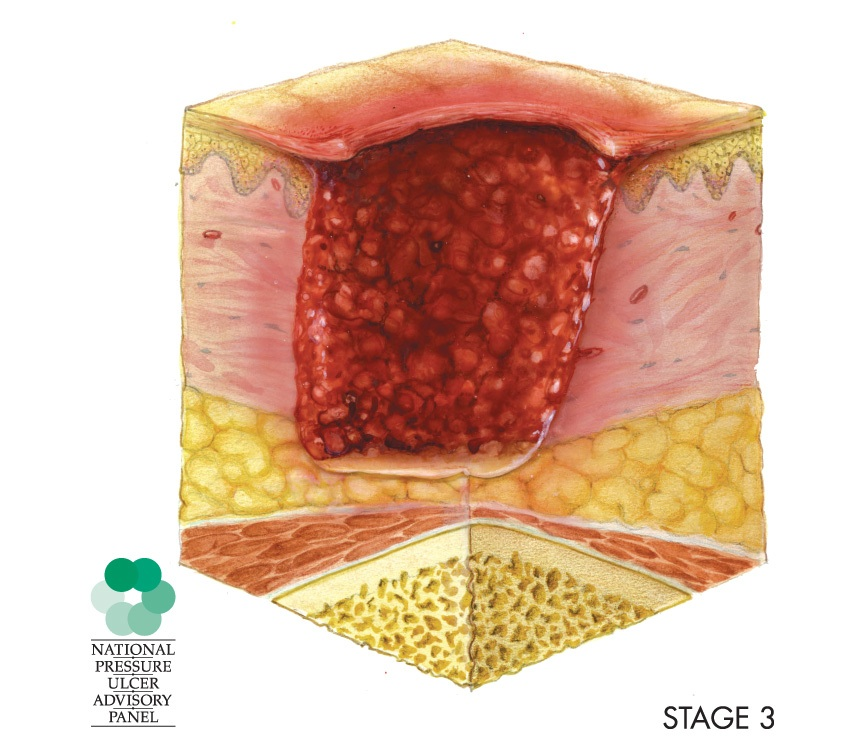
\includegraphics[width=0.3\textwidth]{images/npuap/stage3.png}\label{fig:npuap-stage3}}

			\subfloat[Stage IV]{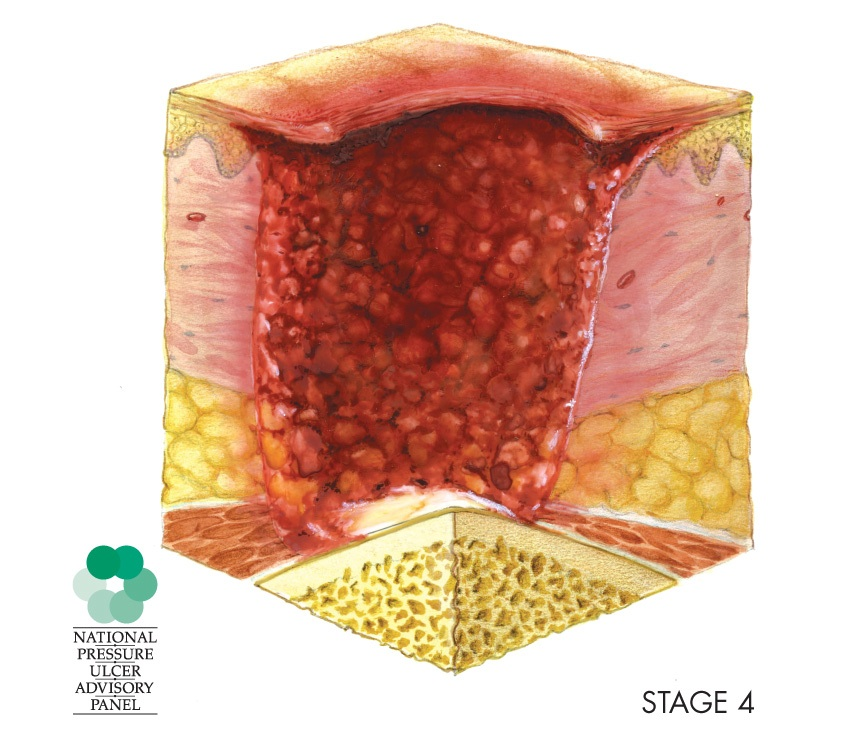
\includegraphics[width=0.3\textwidth]{images/npuap/stage4.png}\label{fig:npuap-stage4}}
			\subfloat[Unstageable]{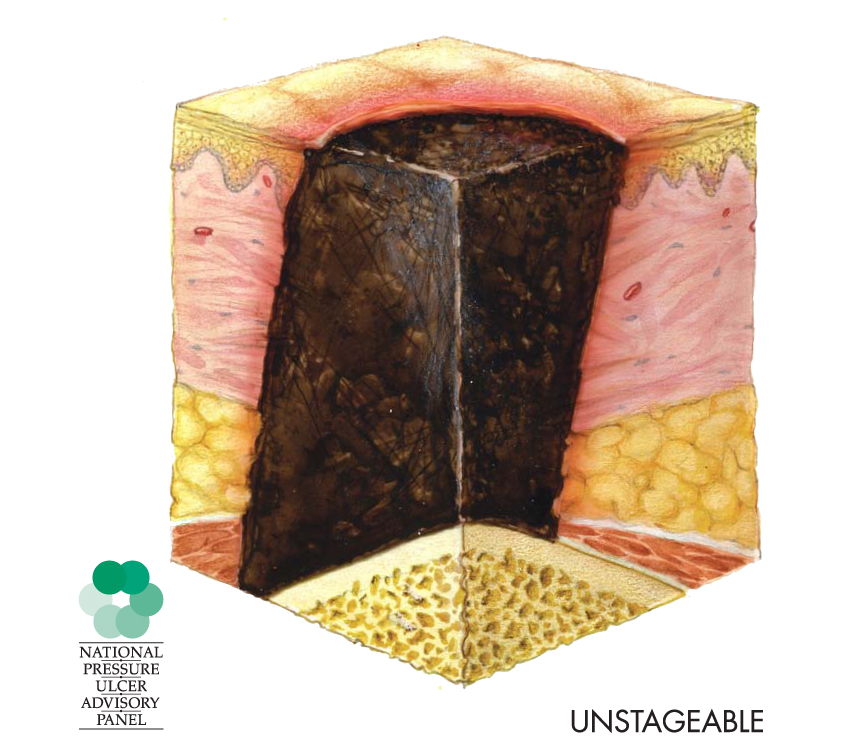
\includegraphics[width=0.3\textwidth]{images/npuap/unstageable.png}\label{fig:npuap-unstageable}}
			\subfloat[Suspected DTI]{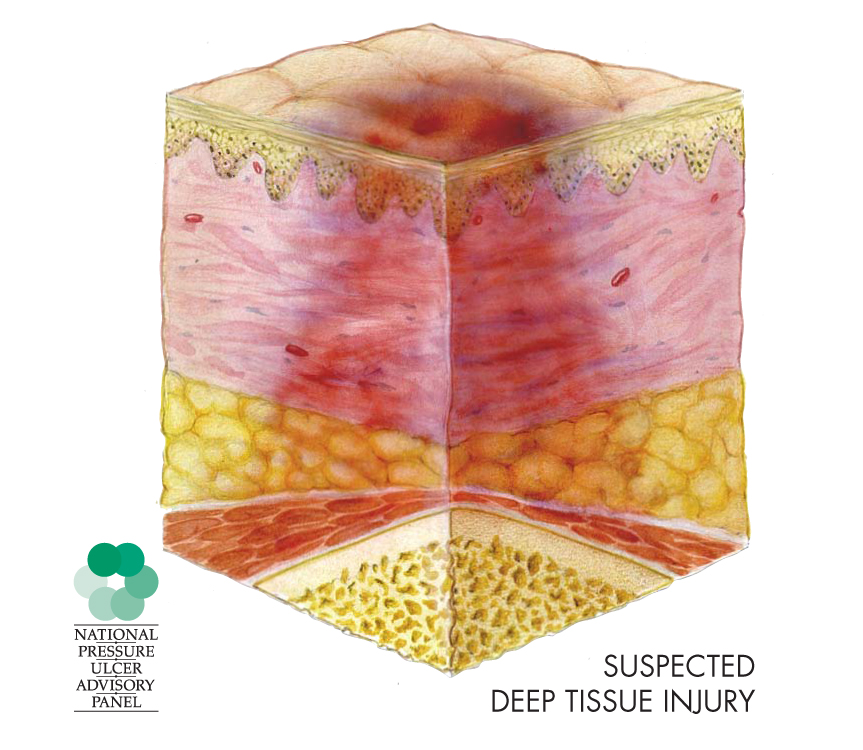
\includegraphics[width=0.3\textwidth]{images/npuap/suspectedDTI.png}\label{fig:npuap-dti}}
			\caption[NPUAUP pressure ulcer staging guidelines]{The NPUAP staging guideline illustrations of the various stages / severities of pressure ulcers.}
			\label{fig:npuap-staging}
		\end{figure*}

		\begin{description}
			\item[Suspected Deep Tissue Injury] \hfill \\
				Purple or maroon localized area of discoloured intact skin or blood-filled blister due to damage of underlying soft tissue from pressure and / or shear. The area may be preceded by tissue that is painful, firm, mushy, boggy, warmer or cooler as compared to adjacent tissue.
			\item[Stage I] \hfill \\
				Intact skin with non-blanchable redness of a localized area usually over a bony prominence. Darkly pigmented skin may not have visible blanching; its colour may differ from the surrounding area.
			\item[Stage II] \hfill \\
				Partial thickness loss of dermis presenting as a shallow open ulcer with a red pink wound bed, without slough. May also present as an intact or open / ruptured serum-filled blister.
			\item[Stage III] \hfill \\
				Full thickness tissue loss. Subcutaneous fat may be visible but bone, tendon or muscle are not exposed. Slough may be present but does not obscure the depth of tissue loss. \emph{May} include undermining and tunnelling.
			\item[Stage IV] \hfill \\
				Full thickness tissue loss with exposed bone, tendon or muscle. Slough or eschar may be present on some parts of the wound bed. Often include undermining and tunnelling.
			\item[Unstageable] \hfill \\
				Full thickness tissue loss in which the base of the ulcer is covered by slough (yellow, tan, grey, green, or brown) and / or eschar (tan, brown or black) in the wound bed.
		\end{description}

		The NPUAP's definitions of pressure ulcers come from clinical experiences with them and are largely based on the ulcer's appearance after they have formed and do not necessarily reflect the true aetiological factors that lead to these conditions. For example, a significant body of literature scientifically describes deep tissue injuries as being much more insidious than a ``localized area of discoloured intact skin'' and suggests that many Stage III and IV pressure ulcers are actually advanced deep tissue injuries rather than advanced Stage I or II ulcers \cite{gefen09}. This chasm between the clinically accepted and scientifically observed definitions of deep tissue injuries is likely due to the lack of any clinical detection ability \cite{campbell10}. What is agreed upon is that deep tissue injuries are a major problem and more needs to be done to facilitate preventing and treating them \cite{black11,maklebust05} and one of the largest hurdles to preventing and treating DTI is the lack of any substantial early detection ability \cite{gunningberg08,milne09}.

		\subsection{Aetiology and Histology}
			\label{sec:litreview-aetiology}
			Deep tissue injuries are thought to occur through the combinatory effects of three distinct but related mechanisms: ischemia, insufficient lymph drainage, and cell deformation. Ischemia is a condition where the blood supply to tissue has been cut off, rendering the tissue unable to function appropriately. Insufficient lymph drainage refers to how waste products may accumulate in tissue when the lymph vessels that normally carry them away become occluded. Cell deformation occurs when mechanical strains are imparted upon the tissue, causing excessive deformation in not only the extracellular matrix, but in the cells as well. Taken together, the presence of these factors has been shown to greatly increase the risk of developing a deep tissue injury \cite{stekelenburg08}.

			For quite some time, ischemia was regarded as the chief acute risk factor for developing late-stage pressure ulcers \cite{witkowski82,dinsdale74,kosiak61}. Although studies have shown that healthy tissue is able to survive complete ischemia for approximately 4 hours before severe necrosis set in \cite{labbe87,strock69}, deep tissue injuries are clinically found when loading times are substantially less than this \cite{aronovitch99,bliss99}. The model of ischemic damage alone could not account for the rate of late-stage pressure ulcers that we were witnessed.

			Once it was realized that ischemia alone could not be the culprit behind deep tissue injury formation, ischemia-induced reperfusion injury became implicated in the formation of DTI \cite{Ytrehus95,Blaisdell02,tsuji05}. An ischemia-induced reperfusion injury is caused when blood is allowed to flow back into a region of tissue that was previously ischemic. While seeming somewhat contrary to its expected effect, the restoration of circulation results in a swelling and inflammatory effect which causes extensive microvascular damage \cite{Blaisdell02}. The effect of reperfusion was confirmed when comparing pure ischemic conditions in tissue to a cycle of ischemic-reperfused conditions over the same period of time, where it was found that significantly greater damage was caused by repeated loading-unloading rather than simple constant loading \cite{tsuji05,salcido94}. While ischemia-reperfusion injuries provide a more complete explanation about the formation of deep tissue injuries, they still do not account for those injuries acquired under constant pressure over short time periods.

			In order for cells to function in a healthy manner, the waste they produce must be constantly carried off and processed via the lymphatic system and its series of lymph vessels that perfuse tissue. If the magnitude of pressure applied to tissue reaches a threshold level, the pressure occludes the lymph vessels and lymphatic drainage ceases \cite{miller81}. Once lymphatic drainage ceases, cell waste accumulates in the tissue and is thought to initiate necrosis in the cells \cite{krouskop78,reddy81,braden87}. Since this model of damage relates to occlusion of vessels, inhibited lymphatic drainage may be categorized as an ischemic risk factor.

			In order to account for deep tissue injuries that form over short time periods, a model of cell deformation leading to necrosis has more recently been proposed \cite{landsman95,bouten01,wang05}. It has constantly been observed that tissue regions which eventually form deep tissue injuries exhibit signs of locally increased strains \cite{stekelenburg06,ceelen08,linderganz08,portnoy09,solis12-03}, with greater degrees of deformation correlating to greater degrees of damage. To account for these results, it has been proposed that excessively deforming strains applied to cells over extended periods of time can alter the permeability of the cell's plasma membranes, leading to an overall reduced cell viability \cite{slomka12}. Further, it has been shown both in finite-element models and experimentally that the stiffness of soft tissue and the corresponding strains that are developed within them are closely related \cite{loerakker13,gefen05,linderganz09,nagel09}. Not only does the amount of deformation depend on the stiffness of tissue, but the stiffness of tissue was found to correlate to the level of deep tissue injury damage seen in the resulting histology \cite{gefen04} with immediate 1.6-fold to 3.3-fold stiffening of the tissue occurring immediately after injury \cite{gefen05,linderganz04}. Further, the stiffness of tissue severely drops below that of healthy tissue when it begins to decompose \cite{gefen05,dimaio01}, leading to a relationship between injury progression and stiffness as shown in Fig. \ref{fig:stiffness-time-relation} (adapted from \cite{gefen09}).

			\begin{figure}[!t]
				\centering
					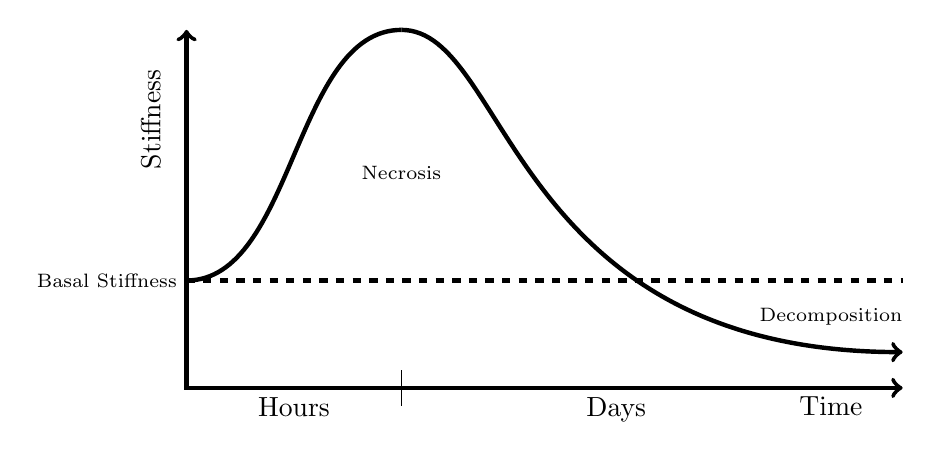
\begin{tikzpicture}[x=0.75\textwidth,y=0.375\textwidth]
						% basal stiffness
						\draw[ultra thick, dashed]
						(0, 0.3) -- (1, 0.3);

						% stiffness curve
						\draw[ultra thick] plot[smooth, tension=1] (0, 0.3) .. controls(0.15, 0.3) and (0.15, 1) .. (0.3, 1);
						\draw[ultra thick, ->] plot[smooth, tension=1] (0.3, 1) .. controls(0.45, 1) and (0.45, 0.1) .. (1, 0.1);

						% axes
						\draw[ultra thick, <->] (0, 1) -- (0, 0) -- (1, 0);

						% time tick
						\draw (0.3, -0.05) -- (0.3, 0.05);

						\node[below] at (0.15, 0) {Hours};
						\node[below] at (0.6, 0) {Days};
						\node[rotate=90] at (-0.05, 0.75) {Stiffness};
						\node[left] at (0, 0.3) {\scriptsize Basal Stiffness};
						\node at (0.3, 0.6) {\scriptsize Necrosis};
						\node at (0.9, 0.2) {\scriptsize Decomposition};
						\node at (0.9, -0.05) {Time};
					\end{tikzpicture}
				\caption[Schematic representation of the time course of tissue stiffness changes in a deep tissue injury site.]{Schematic representation of the time course of tissue stiffness changes in a deep tissue injury site. The estimate for the time-course for local rigor mortis was obtained from animal model studies \cite{portnoy08} and the estimate for the time-course for tissue decomposition was obtained from the forensic literature \cite{dimaio01}. (Adapted from Gefen \cite{gefen09})}
				\label{fig:stiffness-time-relation}
			\end{figure}

			There have been many models of deep tissue injury formation throughout the years, each relating to different mechanisms, though all relating to mechanical stress of the tissue, either through vessel occlusion or direct cellular strain. The truth is most likely a combination of these effects, with cell deformation dominating the damage on shorter time scales with increased applied pressure and vessel occlusion type injuries dominating on longer time scales \cite{stekelenburg08}. In order to further investigate the etiology of PU and DTI, a combination of experimental and numerical studies has been suggested to provide better fundamental knowledge besides existing clinical experience \cite{bouten03}. There is also significant evidence in the literature that suggests that the current NPUAP definitions of PU and DTI are unacceptable and not based on scientific evidence and that updating the clinical definitions to better reflect what exists in the literature is crucial to increasing the success of diagnosis and treatment of PU and DTI \cite{gefen09,campbell10}.

			\comment{
				Other possible papers to cite:
					\cite{ceelen08-8}: Computational model that shows how cells that die under compression decrease in stiffness.
					\cite{gefen07-9}: Review of knowledge of DTI aetiology, and why the NPUAP definition is shitty
					\cite{linderganz06}: Greatest strain occurs deep in the tissue, not at the surface
					\cite{then09}: Material information for examining soft tissue deformation
					\cite{vanNierop10}: Diffusion of water affected only by tissue temperature, not deformation
					\cite{salcido94}: Lesions occur deep in tissue rather than at the surface
					\cite{gefen07}: Sitting posture greatly changes the damage that occurs in PU
					\cite{oomens10}: Interface pressure is not a good measure of tissue health, but rather internal strains are
			}

		\subsection{Detection}

		\comment{While $\mathrm{T}_2^*$-weighted MRI may be used to detect deep tissue damage by detecting oedema in the tissue \cite{loerakker11,stekelenburg06}, it is far from a cost-effective imaging modality for investigating and monitoring DTI in all at-risk patients. }

			\begin{itemize}
				\item Combination of thermographic and ultrasonographic assessments for early detection of deep tissue injury \cite{higashino12}
				\item A review of deep tissue injury development, detection, and prevention \cite{gefen13}
				\item Pressure ulcer knowledge in medical residents: an opportunity for improvement \cite{levine12}
				\item Clinical nurse' knowledge and visual differentiation ability in pressure ulcer classification system and incontinence-associated dermatitis \cite{lee13}
				\item Toward real-time detection of deep tissue injury risk in wheelchair users using Hertz contact theory \cite{agam08}
				\item Compression-induced deep tissue injury examined with magnetic resonance imaging and histology \cite{stekelenburg06}
				\item Low-echoic lesions underneath the skin in subjects with spinal-cord injury \cite{kanno09}
				\item National Pressure Ulcer Advisory Panel's Updated Pressure Ulcer Staging System \cite{black07}
				\item A new pressure ulcer risk assessment scale for individuals with spinal cord injury \cite{salzberg96}
				\item Deep tissue engineering from a bioengineering point of view \cite{gefen09}
				\item Evaluation of four non-invasive methods for examination and characterization of pressure ulcers \cite{andersen08}
				\item Which techniques to improve the early detection and prevention of pressure ulcers? \cite{gehin06}
				\item Inception and validation of a pressure ulcer risk scale in oncology \cite{fromantin11}
				\item Assessment and management of pressure ulcers in the elderly: current strategies \cite{jaul10}
				\item Reliability testing of the national database of nursing quality indicators pressure ulcer indicator \cite{hart10}
				\item Ultrasound assessment of deep tissue injury in pressure ulcers: possible prediction of pressure ulcer progression \cite{aoi08}
				\item 3D ultrasound elastography for early detection of lesions. Evaluation on a pressure ulcer mimicking phantom \cite{deprez07}
			\end{itemize}

		\subsection{Prevention and Treatment}
			\begin{itemize}
				\item \cite{solis12-02}
				\item Prevention of deep tissue injury through muscle contractions induced by intermittent electrical stimulation after spinal cord injury in pigs \cite{solis13}
				\item The importance of internal strain as opposed to interface pressure in the prevention of pressure related deep tissue injury \cite{oomens10}
				\item New methodology for preventing pressure ulcers using actimetry and autonomous nervous system recording \cite{meffre06}
				\item Pressure ulcers: the great insult \cite{maklebust05}
				\item Reaching for the moon: achieving zero pressure ulcer prevalence, an update \cite{bales11}
				\item Distribution of Internal Pressure around Bony Prominences: Implications to deep tissue injury and effectiveness of intermittent electrical stimulation \cite{solis12-02}
				\item Distribution of internal strains around bony prominences in pigs \cite{solis12-03}
				\item Reaching for the moon: achieving zero pressure ulcer prevalence, an update. \cite{bales11}
				\item Reducing pressure ulcers in hip fracture patients \cite{thompson11}
				\item Reducing pressure ulcer prevalence rates in the long-term acute care setting \cite{milne09}
				\item Development of pressure ulcer program across a university health system \cite{carson11}
				\item Assessment and management of pressure ulcers in the elderly: current strategies \cite{jaul10}
				\item Pressure ulcers: the great insult \cite{maklebust05}
				\item Intermittent electrical stimulation redistributes pressure and promotes tissue oxygenation in loaded muscles of individuals with spinal cord injury. \cite{gyawali11}
			\end{itemize}

	\section{Ultrasound Elastography}
		%\lipsum[1]

		\subsection{Quasi-Static Ultrasound Elastography}
			\begin{itemize}
				\item A new method for the visualization and quantification of internal skin elasticity by ultrasound imaging \cite{osanai11}
			\end{itemize}

		\subsection{Acoustic Radiation Force Impulse Imaging}
			\begin{itemize}
				\item derp
			\end{itemize}

		\subsection{Shear Wave Speed Quantification}
			\begin{itemize}
				\item derp
			\end{itemize}

	\section{Numerical Characterization / Finite-Element Modelling}
		%\lipsum[1]

	\section{Conclusion}
		%\lipsum[1]

	\cleardoublepage

	\phantomsection

	\addcontentsline{toc}{section}{References}
	%\bibliographystyle{IEEEtran}
	%\renewcommand{\bibliography}[1]{}
	%\bibliography{references}
	\bibcomplete{references}
	\printbibliography[heading=subbibliography]